\section{Anforderungsanalyse}
\subsection{Anwendungsfalldiagramm}
\begin{figure}[ !h] \centering
%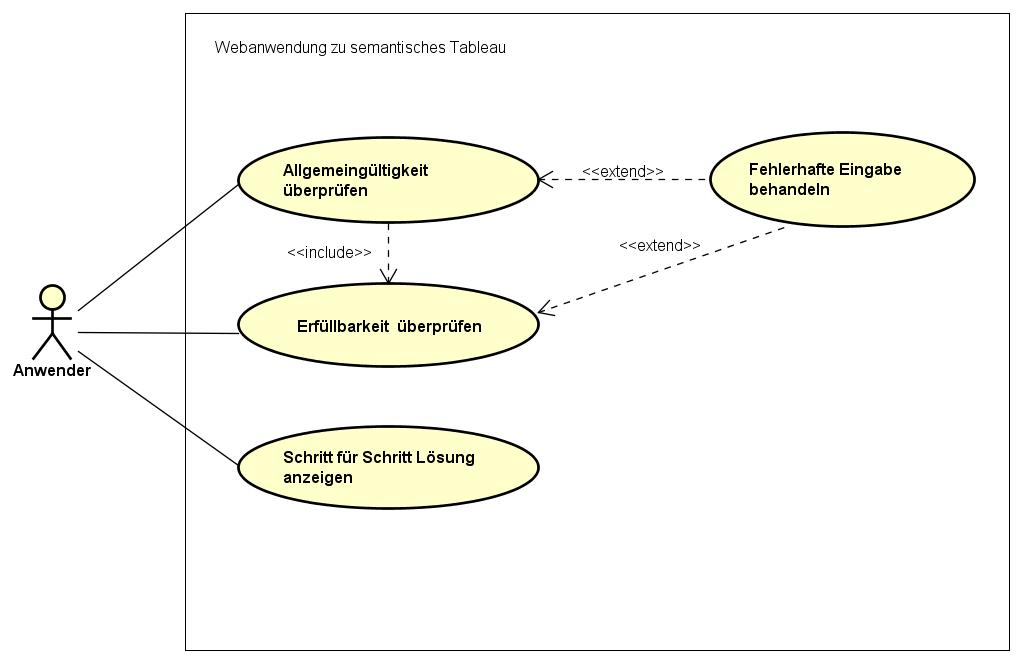
\includegraphics[width=1.0\textwidth,draft=\DraftMode]{UsecaseDiagram}
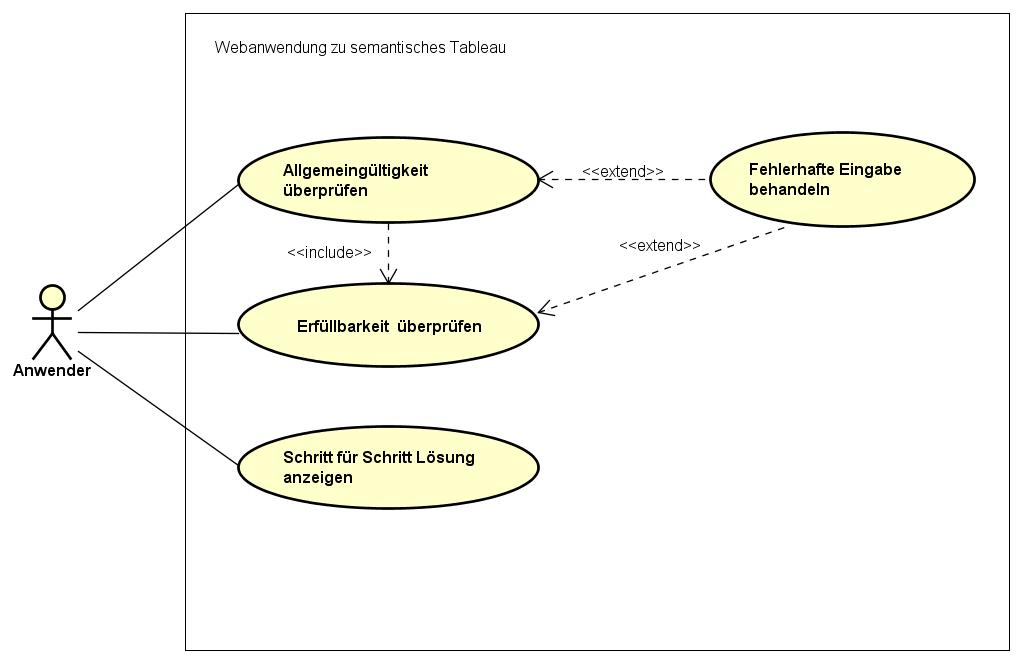
\includegraphics[width=1.0\textwidth]{UsecaseDiagram.jpg}
\caption[Anwendungsfalldiagramm]{Anwendungsfalldiagramm}\label{fig:Anwendungsfalldiagramm}
\end{figure}

\subsection{Anwendungsfallbeschreibung}
\begin{itemize}


%\subsubsection{Anwendungsfall:``Allgemeingültigkeit überprüfen''}
\item \textit{\textbf{Anwendungsfall: ``Allgemeingültigkeit überprüfen''}}

\textbf{Akteure:}

Anwender (initiiert den Anwendungsfall)\\

\textbf{Auslöser:}

Anwender drückt auf ``Tautologie''\\

\textbf{Anfangsbedingungen:}

Der Anwender hat eine Eingabe ins Eingabefeld eingegeben.\\

\textbf{Ereignisfluss:}
\begin{enumerate}
\item Das System prüft, ob die Eingabe ein wohlgeformter Ausdruck der Aussagenlogik ist. 
\item Das System erstellt die Negation der Eingabeformel.
\item Das System zeigt die Darstellung von der Negation der Eingabeformel als Baumstruktur in dem GUI an.
\item Das System initiiert ``Erfüllbarkeit überprüfen'' um zu prüfen, ob die Negation der Eingabeformel erfüllbar ist.
\item Wenn dies erfolgreich ist, erstellt das System das Ergebnis, sodass die Eingabeformel nicht allgemeingültig ist. Wenn nicht, erstellt das System das Ergebnis, sodass die Eingabeformel allgemeingültig ist.
\item Das System zeigt die Darstellung des Tableaus an.
\end{enumerate}

\textbf{Abschlussbedingungen:}

Der Anwender hat entweder das Ergebnis oder eine Systemmeldung über eine fehlerhafte Eingabe erhalten.\\
	
%\subsubsection{Anwendungsfall:``Erfüllbarkeit überprüfen''}
\item \textit{\textbf{Anwendungsfall: ``Erfüllbarkeit überprüfen''}}

\textbf{Akteure:}

Anwender (initiiert den Anwendungsfall)\\

\textbf{Auslöser:}

Anwender drückt auf ``Erfüllbarkeit''\\

\textbf{Anfangsbedingungen:}

Der Anwender hat eine Eingabe ins Eingabefeld eingegeben.\\
 
\textbf{Ereignisfluss:}
\begin{enumerate}
\item Das System prüft, ob die Eingabe ein wohlgeformter Ausdruck der Aussagenlogik ist. 
\item Das System zeigt die Eingabeformel-Darstellung als Baumstruktur in dem GUI an.
\item Das System prüft, ob die Eingabeformel mittels Tableau-Verfahren erfüllbar ist und erstellt das Ergebnis.
\item Das System zeigt die Darstellung des Tableaus an.
\end{enumerate}

\textbf{Abschlussbedingungen:}

Der Anwender hat entweder das Ergebnis oder eine Systemmeldung über eine fehlerhafte Eingabe erhalten.\\

%\subsubsection{Anwendungsfall: ``Schritt für Schritt Lösung auswählen''}
\item \textit{\textbf{Anwendungsfall: ``Schritt für Schritt Lösung anzeigen''}}

\textbf{Akteure:}

Anwender (initiiert den Anwendungsfall)\\

\textbf{Auslöser:}

Anwender drückt auf ``Schritt für Schritt Lösung''\\

\textbf{Anfangsbedingungen:}

Anwender hat ``Erfüllbarkeit'' oder ``Tautologie'' gedrückt.\\

\textbf{Ereignisfluss:}
\begin{enumerate}
\addtolength{\itemindent}{0cm}
\item Das System öffnet ein Pop-up Fenster für die Schritt für Schritt Lösung.
\addtolength{\itemindent}{1cm}
\item  Der Anwender drückt auf ``Nächste Schritt'' um den nächsten Schritt der Lösung anzuzeigen.
\item  Der Anwender drückt auf ``$\times$'' Symbol um das Pop-up Fenster zu schließen.
\addtolength{\itemindent}{0cm}
\end{enumerate}
\begin{enumerate}
  \setcounter{enumi}{3}
 \item Das System schließt das Pop-up Fenster.
\end{enumerate}

\textbf{Abschlussbedingungen:}
Pop-up Fenster ist geschlossen. Der Anwender kann die vorherige Formel nochmal prüfen oder eine neue Formel eingeben.\\

%\textbf{Anwendungsfall:}  "Tableau anzeigen"
%\textbf{Akteure:}
%- System (initiiert den Anwendungsfall)
%-Google Chart Tools (stellt das Tableau dar)
%\textbf{Auslöser:}
%Das System initiiert " Tableau darstellen " zur Darstellung des Tableaus.
%\textbf{Anfangsbedingungen:}
%Das System hat das Tableau erstellt.
%\textbf{Ereignisfluss:}
%1.	Das System prüft, ob die Eingabe ein wohlgeformter Ausdruck der Aussagenlogik ist. 
%2.	Das System prüft, ob die Eingabe Formel mittels Tableau-Verfahren erfüllbar ist und erstellt das Ergebnis.
%3.	Das System initiiert " Tableau darstellen " zur Darstellung des Tableaus.
%\textbf{Abschlussbedingungen:}
%Die Tableau-Darstellung müssen innerhalb von 5 Sekunden bereitgestellt werden können.
%\textbf{Qualitätsanforderung:}

%\subsubsection{Anwendungsfall: ``Fehlerhafte Eingabe behandeln''}
\item \textit{\textbf{Anwendungsfall: ``Fehlerhafte Eingabe behandeln''}}

\textbf{Akteure:}

System (initiiert den Anwendungsfall)\\

\textbf{Auslöser:}

Dieser Anwendungsfall erweitert die Anwendungsfälle ``Allgemeingültigkeit überprüfe'' und ``Erfüllbarkeit überprüfen''. Es wird vom System initiiert, sobald die Eingabe nicht ein wohlgeformter Ausdruck der Aussagenlogik ist.\\

\textbf{Anfangsbedingungen:}

Anwender hat eine fehlerhafte Eingabe eingegeben.\\

\textbf{Ereignisfluss:}
\begin{enumerate}
\item Das System gibt eine Systemmeldung aus.
\end{enumerate}

\textbf{Abschlussbedingungen:}

Der Anwender erhält eine Systemmeldung und kann die Eingabe korrigieren.\\

\end{itemize}
